% Generado por trabajo_en_curso/week5/latex/convertir.py a partir del .docx de la memoria.
% A partir de ahora este fichero es la fuente: edítalo directamente.

\chapter{Planificación}\label{sec:2}

\needspace{6\baselineskip}
\section{Datos globales del proyecto}\label{sec:2-1}

El inicio se sitúa el 19 de octubre de 2026, tras finalizar la fase GEP. Esta decisión evita solapar entregables académicos y permite dedicar el periodo posterior a la construcción, validación y redacción. La fecha límite operativa es el 10 de enero de 2027; por tanto, la validación funcional se completa antes de la última semana.

\begin{table}[H]
\centering\small
\begin{tabularx}{\textwidth}{>{\hsize=0.957\hsize\raggedright\arraybackslash}X>{\hsize=1.043\hsize\raggedright\arraybackslash}X}
\toprule
\rowcolor{cabeceratabla} \textbf{Parámetro} & \textbf{Valor} \\
\midrule
Inicio planificado & 19/10/2026 \\
Finalización y defensa interna & 10/01/2027 \\
Duración calendario & 12 semanas \\
Carga de trabajo base & 405 horas \\
Reserva de contingencia & 45 horas (11,1 \% de la base) \\
Dedicación prevista & 37,5 horas semanales de media \\
Método de ejecución & 4 sprints de 3 semanas \\
Hitos & Requisitos, CRM seleccionado, prototipo, validación y cierre \\
\bottomrule
\end{tabularx}
\caption{Parámetros de planificación}\label{tab:8}
\end{table}

\needspace{6\baselineskip}
\subsection{Criterios de estimación}\label{sec:2-1-1}

Las estimaciones se expresan en horas y se han descompuesto en tareas de tamaño manejable. Las tareas de construcción se han dimensionado entre 14 y 45 horas, manteniéndose por debajo del umbral de 50 horas. La suma de tareas ordinarias es 405 horas. Las 45 horas de contingencia se mantienen diferenciadas del trabajo base, pero forman parte de la capacidad total planificada de 450 horas. Esto sumado a las 90 horas de GEP dan un total de 540 horas de TFG.

\needspace{6\baselineskip}
\subsection{Seguimiento}\label{sec:2-1-2}

Al cierre de cada semana se actualizarán horas reales, tareas terminadas, impedimentos y fecha estimada de los hitos. Al final de cada sprint se realizará una revisión del incremento: primero requisitos y selección, después configuración, posteriormente adaptación de módulos y finalmente pruebas. Si una tarea crítica se retrasa más de cuatro horas, se aplicará el plan alternativo correspondiente.

\needspace{6\baselineskip}
\subsection{Calendario y dedicación}\label{sec:2-1-3}

El calendario considera la disponibilidad del estudiante, los festivos previsibles y la necesidad de reservar las validaciones con terceros fuera del periodo navideño. La carga base equivale a 33,75 horas semanales y la contingencia reserva 3,75 horas semanales de capacidad no asignada. La dedicación total prevista es, por tanto, de 37,5 horas semanales. Esta distribución permite que los hitos tengan evidencia disponible antes de la revisión de cada sprint y evita concentrar la memoria técnica al final del proyecto.

\needspace{6\baselineskip}
\section{Especificación y descripción de tareas}\label{sec:2-2}

La EDT se organiza en siete paquetes: gestión, análisis, selección, diseño y configuración, adaptación, validación y cierre. Las precedencias se indican con la notación Tn \textless{} Tm, que significa que la tarea Tn debe finalizar antes de iniciar Tm. Los recursos son el estudiante, la dirección y tutoría, usuarios de validación y un entorno de pruebas con SuiteCRM.

\begin{table}[H]
\centering\footnotesize
\begin{tabularx}{\textwidth}{>{\hsize=0.500\hsize\raggedright\arraybackslash}X>{\hsize=2.223\hsize\raggedright\arraybackslash}X>{\hsize=0.260\hsize\raggedright\arraybackslash}X>{\hsize=0.874\hsize\raggedright\arraybackslash}X>{\hsize=1.144\hsize\raggedright\arraybackslash}X}
\toprule
\rowcolor{cabeceratabla} \textbf{Código} & \textbf{Tarea} & \textbf{h} & \textbf{Precedencia} & \textbf{Recursos} \\
\midrule
T1 & Planificación detallada, seguimiento semanal y control de cambios & 25 & — & Estudiante, dirección \\
T2 & Definir actores, necesidades y casos de uso del centro & 18 & — & Estudiante, usuarios \\
T3 & Modelar proceso actual, requisitos y protección de datos & 28 & T2 & Estudiante, usuarios \\
T4 & Establecer criterios, preselección y pruebas de concepto CRM & 16 & T3 & Estudiante, fuentes técnicas \\
T5 & Comparar candidatos y justificar la selección de SuiteCRM & 16 & T4 & Estudiante, entorno de prueba \\
T6 & Diseñar modelo de datos, roles, permisos y trazabilidad & 30 & T3 \textless{} T6; T5 \textless{} T6 & Estudiante, dirección \\
T7 & Preparar instancia, entorno de desarrollo y configuración base & 22 & T5 \textless{} T7 & Estudiante, entorno SuiteCRM \\
T8 & Configurar inscripción, actividades y control de asistencia & 30 & T6 \textless{} T8; T7 \textless{} T8 & Estudiante, SuiteCRM \\
\bottomrule
\end{tabularx}
\caption{Paquetes de trabajo y tareas (parte 1)}\label{tab:9}
\end{table}

T1 y la documentación (T14) son tareas transversales: se ejecutan durante toda la planificación y generan evidencia para el seguimiento. La selección del CRM termina antes de configurar la plataforma, pero el modelo de procesos puede avanzar en paralelo con el análisis de candidatos.

\needspace{6\baselineskip}
\subsection{Paquetes de trabajo}\label{sec:2-2-1}

El primer paquete transforma el escenario de referencia en necesidades verificables. El segundo compara CRM con criterios funcionales, técnicos y de protección de datos. Una vez seleccionada la plataforma, los paquetes de diseño y adaptación convierten los requisitos en configuraciones y extensiones concretas. La validación se realiza sobre casos de prueba que reproducen una sesión de actividad extraescolar: alta, asistencia, entrega y comunicación de una incidencia.

\needspace{6\baselineskip}
\subsection{Criterio de descomposición}\label{sec:2-2-2}

Cada tarea se ha formulado como una acción con un resultado comprobable. Las tareas transversales se mantienen separadas de las tareas funcionales para no ocultar el esfuerzo de seguimiento y documentación. Esta descomposición facilita asignar horas, reconocer las dependencias reales y replanificar una tarea sin alterar artificialmente el resto de la EDT~\cite{ref19}.

\begin{table}[H]
\centering\footnotesize
\begin{tabularx}{\textwidth}{>{\hsize=0.500\hsize\raggedright\arraybackslash}X>{\hsize=2.290\hsize\raggedright\arraybackslash}X>{\hsize=0.270\hsize\raggedright\arraybackslash}X>{\hsize=0.874\hsize\raggedright\arraybackslash}X>{\hsize=1.066\hsize\raggedright\arraybackslash}X}
\toprule
\rowcolor{cabeceratabla} \textbf{Código} & \textbf{Tarea} & \textbf{h} & \textbf{Precedencia} & \textbf{Recursos} \\
\midrule
T9 & Implementar custodia, autorizaciones y comprobaciones de entrega & 36 & T6 \textless{} T9; T7 \textless{} T9 & Estudiante, SuiteCRM \\
T10 & Implementar incidencias, prioridad, escalado y comunicación & 30 & T6 \textless{} T10; T7 \textless{} T10 & Estudiante, SuiteCRM \\
T11 & Diseñar pruebas funcionales, de permisos y datos sintéticos & 20 & T8 \textless{} T11; T9 \textless{} T11; T10 \textless{} T11 & Estudiante, usuarios \\
T12 & Ejecutar pruebas integradas y corregir defectos priorizados & 28 & T11 & Estudiante, entorno SuiteCRM \\
T13 & Validar prototipo y consolidar retroalimentación & 14 & T12 & Estudiante, usuarios \\
T14 & Documentar decisiones, resultados y evidencias de forma continua & 32 & — & Estudiante \\
T15 & Redactar memoria final, anexos, guía técnica y manual de uso & 45 & T13; T14 & Estudiante, dirección \\
T16 & Revisión final, entrega y preparación de defensa & 15 & T15 & Estudiante, dirección \\
\bottomrule
\end{tabularx}
\caption{Paquetes de trabajo y tareas (parte 2)}\label{tab:10}
\end{table}

La ruta que puede comprometer la fecha final es: requisitos (T2-T3), selección (T4-T5), diseño y configuración (T6-T7), adaptación (T8-T10), pruebas (T11-T13) y cierre (T15-T16). T14 tiene holgura porque se realiza en paralelo, aunque su contenido debe estar actualizado antes de T15. La EDT suma 405 horas de trabajo base.

\begin{figure}[htbp]
\centering
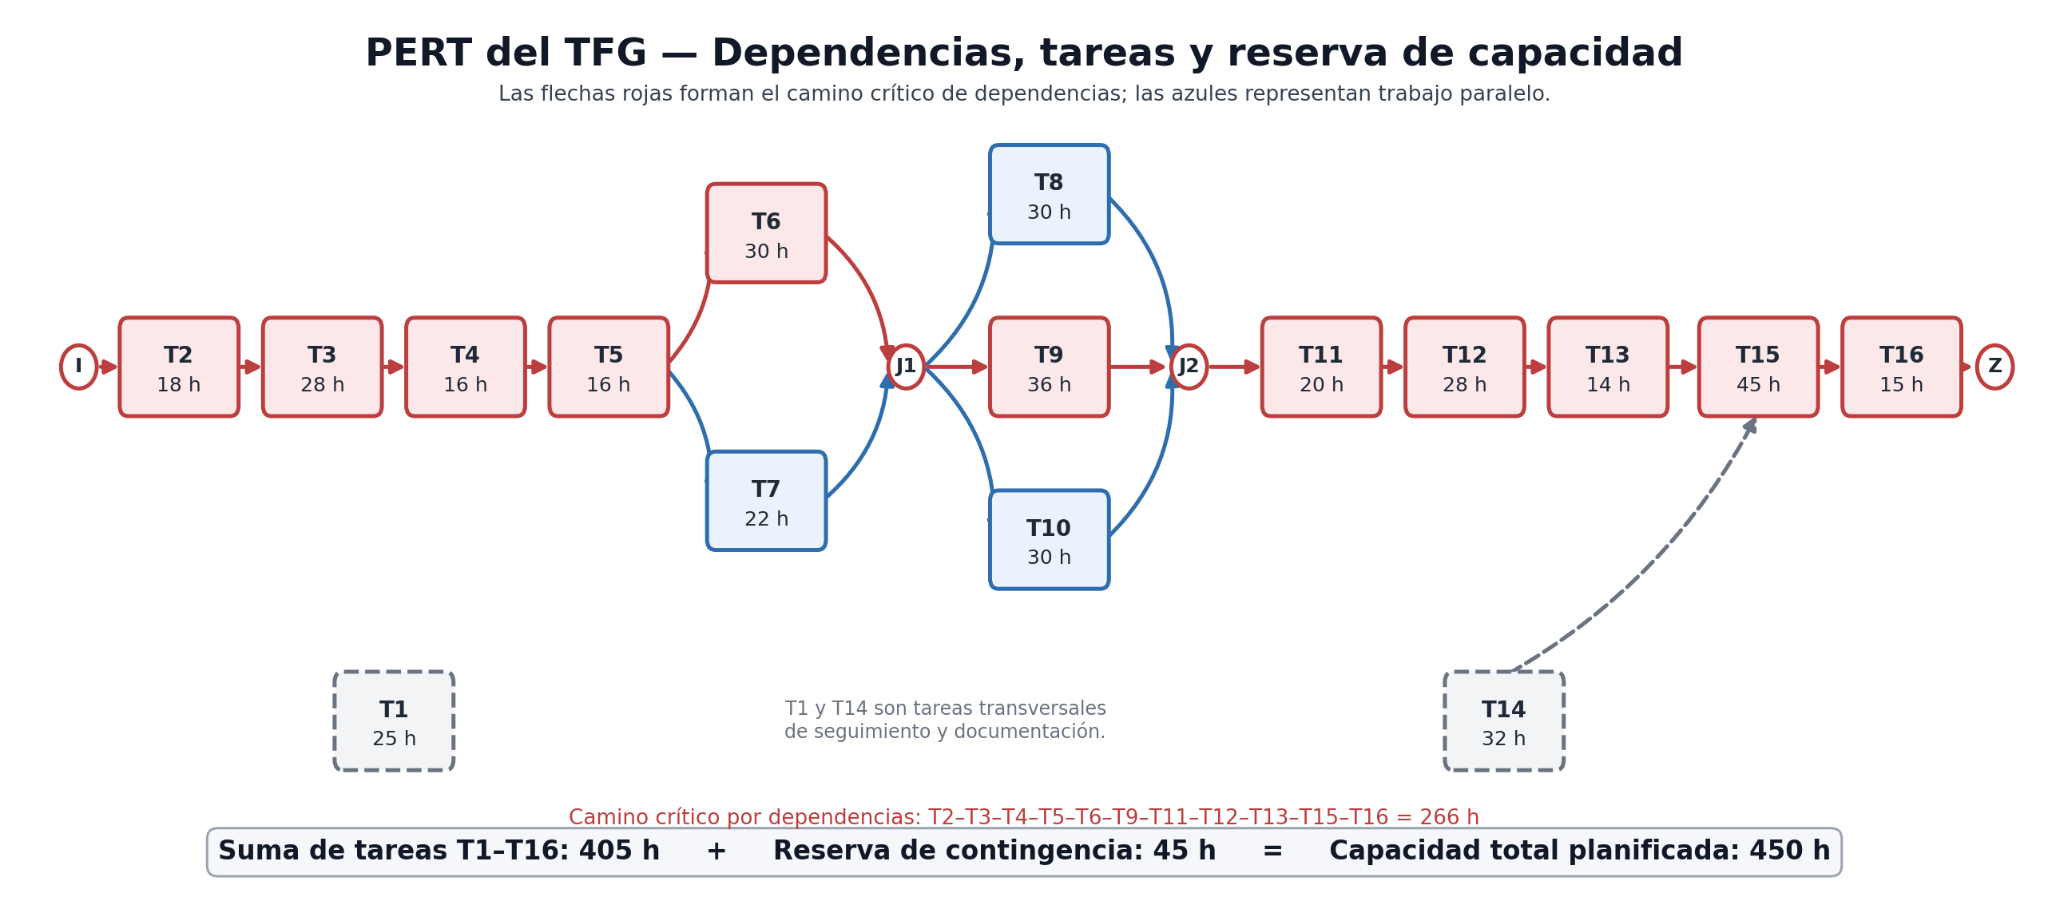
\includegraphics[width=\textwidth]{imagenes/pert.png}
\caption[PERT simplificado y dependencias principales]{PERT simplificado y dependencias principales. La ruta superior representa el camino crítico de referencia}\label{fig:1}
\end{figure}

\needspace{6\baselineskip}
\subsection{Recursos y control de la carga}\label{sec:2-2-3}

El estudiante ejecuta las tareas de análisis, diseño, configuración, desarrollo, pruebas y documentación. La dirección y tutoría aportan contraste metodológico en los hitos; los usuarios de validación revisan la adecuación de los flujos. El entorno de pruebas evita manipular datos reales de menores. Las tareas de mayor esfuerzo son T9, T10 y T15; se han dividido funcionalmente para que el control semanal pueda detectar cualquier desviación.

\needspace{6\baselineskip}
\section{Planificación temporal y diagrama de Gantt}\label{sec:2-3}

El Gantt representa el calendario base de 405 horas y la capacidad de contingencia de 45 horas. Las actividades se ejecutan dentro del intervalo mostrado según las dependencias de las Tablas~\ref{tab:9} y~\ref{tab:10}. Las líneas verticales separan los sprints S1-S4. Gestión y documentación se desarrollan de forma continua; esta concurrencia permite mantener trazabilidad y detectar desviaciones pronto~\cite{ref18,ref20}.

\begin{figure}[htbp]
\centering
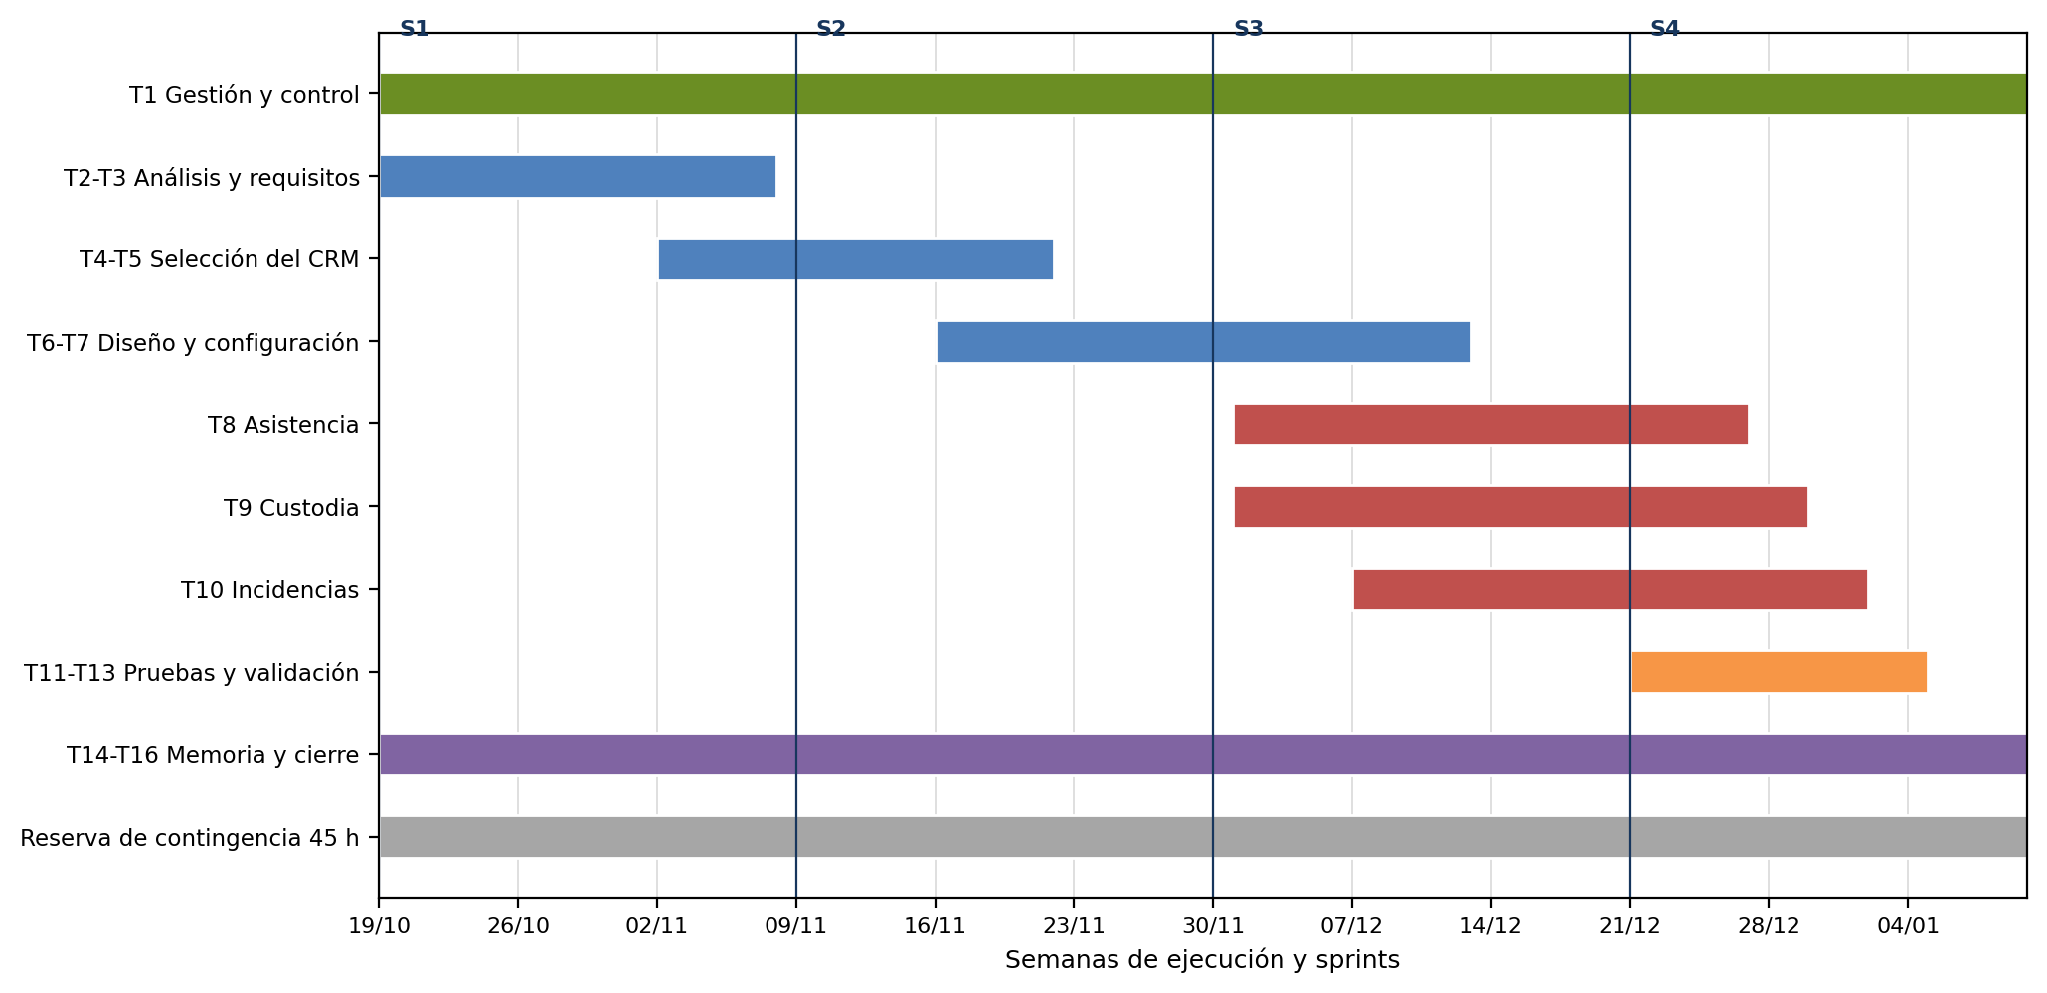
\includegraphics[width=\textwidth]{imagenes/gantt.png}
\caption[Diagrama de Gantt por sprints]{Diagrama de Gantt por sprints. El plan reserva 45 horas de capacidad de contingencia dentro del calendario}\label{fig:2}
\end{figure}

\needspace{12\baselineskip}
\subsection{Hitos de control}\label{sec:2-3-1}

\begin{table}[H]
\centering\small
\begin{tabularx}{\textwidth}{>{\hsize=0.525\hsize\raggedright\arraybackslash}X>{\hsize=1.475\hsize\raggedright\arraybackslash}X}
\toprule
\rowcolor{cabeceratabla} \textbf{Fecha} & \textbf{Resultado verificable} \\
\midrule
H1 · 08/11 & Requisitos y procesos validados \\
H2 · 22/11 & CRM seleccionado y justificado \\
H3 · 13/12 & Modelo, permisos y configuración base listos \\
H4 · 02/01 & Módulos de asistencia, custodia e incidencias adaptados \\
H5 · 05/01 & Pruebas y validación funcional completadas \\
H6 · 10/01 & Memoria cerrada y entrega preparada \\
\bottomrule
\end{tabularx}
\caption{Hitos de control}\label{tab:11}
\end{table}

\needspace{6\baselineskip}
\subsection{Lectura del calendario}\label{sec:2-3-2}

S1 concentra la definición y el contraste del alcance. S2 finaliza la selección y prepara la plataforma. S3 produce los tres módulos prioritarios y comienza las pruebas. S4 cierra la validación, consolida la memoria y deja margen para la revisión final. La carga semanal total es 37,5 horas: 33,75 horas de trabajo base y 3,75 horas no asignadas para contingencias. El periodo navideño se reserva para trabajo individual de construcción y documentación; no se sitúan en él validaciones que dependan de terceros.

\needspace{6\baselineskip}
\subsection{Seguimiento y replanificación}\label{sec:2-3-3}

El Gantt constituye la línea base del proyecto: relaciona tareas, fechas, hitos y dependencias~\cite{ref16,ref17}. La planificación se actualizará con datos reales una vez por semana. No se modificará la fecha final sin evaluar antes el camino crítico, la reserva disponible y los hitos afectados. De este modo se conserva una diferencia visible entre el plan inicial y la ejecución real.

\needspace{6\baselineskip}
\subsection{Indicadores de control por sprint}\label{sec:2-3-4}

Cada revisión semanal compara la situación prevista con la real. Los indicadores no sustituyen al juicio del proyecto, pero permiten decidir si basta con reajustar el orden de trabajo o si es necesario activar una reserva. El avance se comunica en términos de productos verificables, no solo de porcentaje de tiempo consumido.

\begin{table}[H]
\centering\small
\begin{tabularx}{\textwidth}{>{\hsize=1.054\hsize\raggedright\arraybackslash}X>{\hsize=1.404\hsize\raggedright\arraybackslash}X>{\hsize=0.542\hsize\raggedright\arraybackslash}X}
\toprule
\rowcolor{cabeceratabla} \textbf{Indicador} & \textbf{Uso de la información} & \textbf{Frecuencia} \\
\midrule
Horas reales / planificadas & Detectar sobreesfuerzo o subestimación & Semanal \\
Tareas completadas / previstas & Medir cumplimiento del sprint & Semanal \\
Dependencias bloqueadas & Identificar impactos en el camino crítico & Semanal \\
Defectos críticos abiertos & Decidir prioridad de corrección & En pruebas \\
Hitos alcanzados & Confirmar productos verificables & Fin de sprint \\
\bottomrule
\end{tabularx}
\caption{Indicadores de seguimiento}\label{tab:12}
\end{table}

\needspace{12\baselineskip}
\subsection{Cadencia de trabajo}\label{sec:2-3-5}

\begin{table}[H]
\centering\small
\begin{tabularx}{\textwidth}{>{\hsize=0.433\hsize\raggedright\arraybackslash}X>{\hsize=1.567\hsize\raggedright\arraybackslash}X}
\toprule
\rowcolor{cabeceratabla} \textbf{Momento} & \textbf{Actividad de control} \\
\midrule
Lunes & Actualizar el tablero, planificar la semana y priorizar tareas críticas. \\
Mitad de semana & Revisar avance, registrar impedimentos y consultar dudas técnicas. \\
Fin de semana & Comparar horas, actualizar Gantt y preparar evidencia documental. \\
Fin de sprint & Validar el incremento, revisar riesgos y aprobar la siguiente iteración. \\
\bottomrule
\end{tabularx}
\caption{Cadencia de trabajo}\label{tab:13}
\end{table}

Esta cadencia refuerza el carácter iterativo del plan: cada sprint produce un resultado revisable y actualiza las estimaciones de las tareas posteriores sin perder la trazabilidad del calendario base.

\needspace{6\baselineskip}
\section{Gestión de riesgos y planes alternativos}\label{sec:2-4}

Los riesgos se gestionan mediante revisión semanal. Cuando un riesgo se active, se registrará la desviación y se aplicará la respuesta indicada. La reducción de alcance solo se contempla como última medida y nunca afectará a los tres procesos de seguridad infantil: asistencia, custodia e incidencias.

\begin{table}[H]
\centering\footnotesize
\begin{tabularx}{\textwidth}{>{\hsize=0.500\hsize\raggedright\arraybackslash}X>{\hsize=1.195\hsize\raggedright\arraybackslash}X>{\hsize=0.575\hsize\raggedright\arraybackslash}X>{\hsize=1.087\hsize\raggedright\arraybackslash}X>{\hsize=1.643\hsize\raggedright\arraybackslash}X}
\toprule
\rowcolor{cabeceratabla} \textbf{Riesgo} & \textbf{Descripción} & \textbf{Prob. / impacto} & \textbf{Prevención} & \textbf{Plan alternativo} \\
\midrule
R1 & Cambios o ambigüedad en las autorizaciones de recogida & Media / Alta & Prototipo temprano y validación de reglas. & Congelar reglas mínimas y usar 12 h de reserva para adaptar formularios. \\
R2 & Complejidad no prevista al extender SuiteCRM & Media / Alta & Prueba técnica en S2 y módulos pequeños. & Sustituir automatismo no esencial por flujo configurado; reserva de 16 h. \\
R3 & Disponibilidad limitada de usuarios para validar & Alta / Media & Acordar sesiones y casos de prueba con antelación. & Validación asíncrona con guion y evidencia; reserva de 8 h. \\
R4 & Defectos detectados cerca del cierre & Media / Alta & Pruebas por módulo desde S3. & Priorizar defectos críticos y usar 9 h de reserva; mantener H5 como límite. \\
\bottomrule
\end{tabularx}
\caption{Riesgos y respuesta planificada}\label{tab:14}
\end{table}

\needspace{6\baselineskip}
\subsection{Viabilidad del plan alternativo}\label{sec:2-4-1}

La reserva total de 45 horas se distribuye sólo tras comprobar que la desviación amenaza una tarea crítica. Se conserva como capacidad no asignada de 3,75 horas semanales y se utiliza por el estudiante en el entorno local; la directora aprueba cualquier uso superior a ocho horas o que afecte a una regla de seguridad. R1 activa 12 horas si una regla de recogida resulta ambigua o incompatible durante el contraste; R2 activa 16 horas si la prueba técnica impide resolver una personalización crítica; R3 activa 8 horas si no se consigue una sesión de validación; y R4 activa 9 horas si queda un defecto crítico antes de H5. En todos los casos se preservan asistencia, custodia e incidencias. Solo se posponen mejoras no esenciales portal familiar, indicadores ampliados o automatismos no críticos, sin desplazar H5 ni H6.

\needspace{6\baselineskip}
\subsection{Criterio de escalado}\label{sec:2-4-2}

Una desviación de hasta cuatro horas se corrige dentro del sprint y se registra en el seguimiento. Entre cuatro y ocho horas se revisa la secuencia de tareas y se usa la parte de reserva asociada al riesgo. Si supera ocho horas, afecta a la protección de datos o obliga a cambiar una regla de custodia, se consulta a la directora antes de continuar. El alcance se mantiene estable, solo podrían posponerse mejoras de usabilidad, el portal familiar, indicadores ampliados o automatismos no críticos; nunca el control de asistencia, la trazabilidad de custodia ni la gestión de incidencias.

